\chapter{Nanometer-Resolved Imaging Vibrometer}

Conventional laser vibrometers are incapable of performing multi-dimensional vibrometry at high speeds because they build on single-point measurements and rely on beam scanning, significantly limiting their utility and precision. Here we introduce a laser vibrometer that performs high-speed multi-dimensional imaging-based vibration and velocity measurements with nanometer-scale axial resolution without the need for beam scanning. As a proof-of-concept, we demonstrate real-time microscopic imaging of acoustic vibrations with 1 nm axial resolution, 1200 image pixels, and 30 ps dwell time at 36.7 MHz scan rate.

\section{Introduction}

Laser vibrometry is a powerful tool for measuring surface vibrations and displacements in a non-contact and non-invasive manner. It has been used in a diverse range of scientific \cite{castellini2006laser,broch1980mechanical}, industrial \cite{castellini2006laser,broch1980mechanical,drain1980laser,arnott1990laser}, and biomedical \cite{castellini2006laser,drain1980laser,goode1996laser,huber2001evaluation} applications. Common industrial applications include non-destructive inspection and diagnosis of aircraft components, musical instruments, hard disk drives, microelectromechanical systems (MEMS), and automotive brakes \cite{castellini2006laser,broch1980mechanical,drain1980laser}. Furthermore, laser vibrometers are widely employed in biological research and clinical environments for diagnosis of tympanic membranes \cite{goode1996laser,huber2001evaluation}, observation of insect communication \cite{castellini2006laser,drain1980laser}, and evaluation of dental instruments \cite{castellini2006laser,drain1980laser}.

Unfortunately, conventional methods for laser vibrometry such as laser Doppler vibrometry1-6 are unable to perform imaging based vibration measurements at high speeds. This is because their operation builds on single-point measurements and relies on beam scanning for multi-dimensional laser vibrometry. In other words, the scan rate of conventional multi-dimensional laser vibrometers (also called scanning vibrometers) is limited by that of laser scanners although the single-point measurement itself is fast (on the order of $\sim$10 MHz or higher). Currently, the maximum scan rates provided by commercially available laser scanners (e.g., galvanometric mirrors \cite{conant2002micromachined} and acousto-optic deflectors \cite{pape1994design}) are $\sim$100 kHz in 1D line scans and $\sim$1 kHz in two-dimensional (2D) raster or spiral scans. This speed limitation significantly restricts the utility and precision of laser vibrometers, especially in high-speed vibrometry applications including MEMS devices and impact analysis \cite{castellini2006laser,broch1980mechanical,drain1980laser}.

Efforts have been made to mitigate the speed limitation in multi-dimensional laser vibrometers. One of the popular methods is the illumination of the target with multiple laser beams \cite{zheng1998multichannel,fu2010spatially}, but the number of image pixels is significantly limited (typically up to $\sim$10) \cite{zheng1998multichannel,fu2010spatially} by the complexity and cost of the required optical components (e.g., multiple lasers, interferometers, and photodetectors). Another type of vibrometer that does not require beam scanning relies on the use of an array detector [i.e., the complementary metal–oxide–semiconductor (CMOS) camera] \cite{popescu2006optical}, and hence its scan rate is limited by the frame rate of the camera (up to $\sim$10 kHz) \cite{popescu2006optical} and also the trade-off between the number of pixels and frame rate.

In this chapter, we propose and demonstrate a laser vibrometer that overcomes the limitations in the conventional multi-dimensional laser vibrometers and achieves high-speed imaging-based surface vibration measurements with nanometer-scale axial resolution at $\sim$100 times higher scan rates than the conventional methods. This method is an extension of the recently developed ultrafast imaging technology known as serial time-encoded amplified imaging/microscopy (STEAM) \cite{goda2009serial,goda2008amplified,qian2009real} to depth-resolved multi-dimensional imaging. By stretching in time a spectrally coded image, this method does not require beam scanning for multi-dimensional vibrometry. Furthermore, the superior temporal resolution of this method also enables multi-dimensional velocimetry as the velocity of the surface can be obtained from the axial position of the surface. The method’s fast shutter speed (dwell time) ensures nearly-instantaneous frame acquisition and eliminates image blurring. As a proof-of-concept, we demonstrate real-time depth-resolved imaging of acoustic vibrations up to 30 kHz with 1 nm axial resolution, 1200 image pixels, and 30 ps dwell time at 36.7 MHz scan rate.

An experimental apparatus of the proposed method, which we refer to as STEAM vibrometry, is shown in Figure \ref{fig:APL2011_Figure1}. The optical source is a mode-locked femtosecond pulse fiber laser with a pulse repetition rate of 36.7 MHz. After supercontinuum generation in a highly nonlinear fiber and band-pass filtering, a nearly flat spectral shape with $\sim$20 nm bandwidth centered at 1590 nm is produced for target illumination. A pair of diffraction gratings with 1100 lines/mm spatially disperses the pulses along a 1D line, which are directed toward the vibrating target. The reflected pulses are interfered with the reference pulses in a Michelson interferometer, resulting in the spectral interference between the test and reference pulses. Here the lateral and axial coordinates of the target are encoded into the different frequencies and corresponding amplitudes of each back-reflected spatially dispersed pulse, respectively. This situation may be better understood by interpreting the optical configuration in such a way that multiple continuous-wave lasers are incident onto different spatial coordinates of the target in a shared Michelson interferometer with their longitudinal modes locked.

\begin{figure}[htb!]
\centering
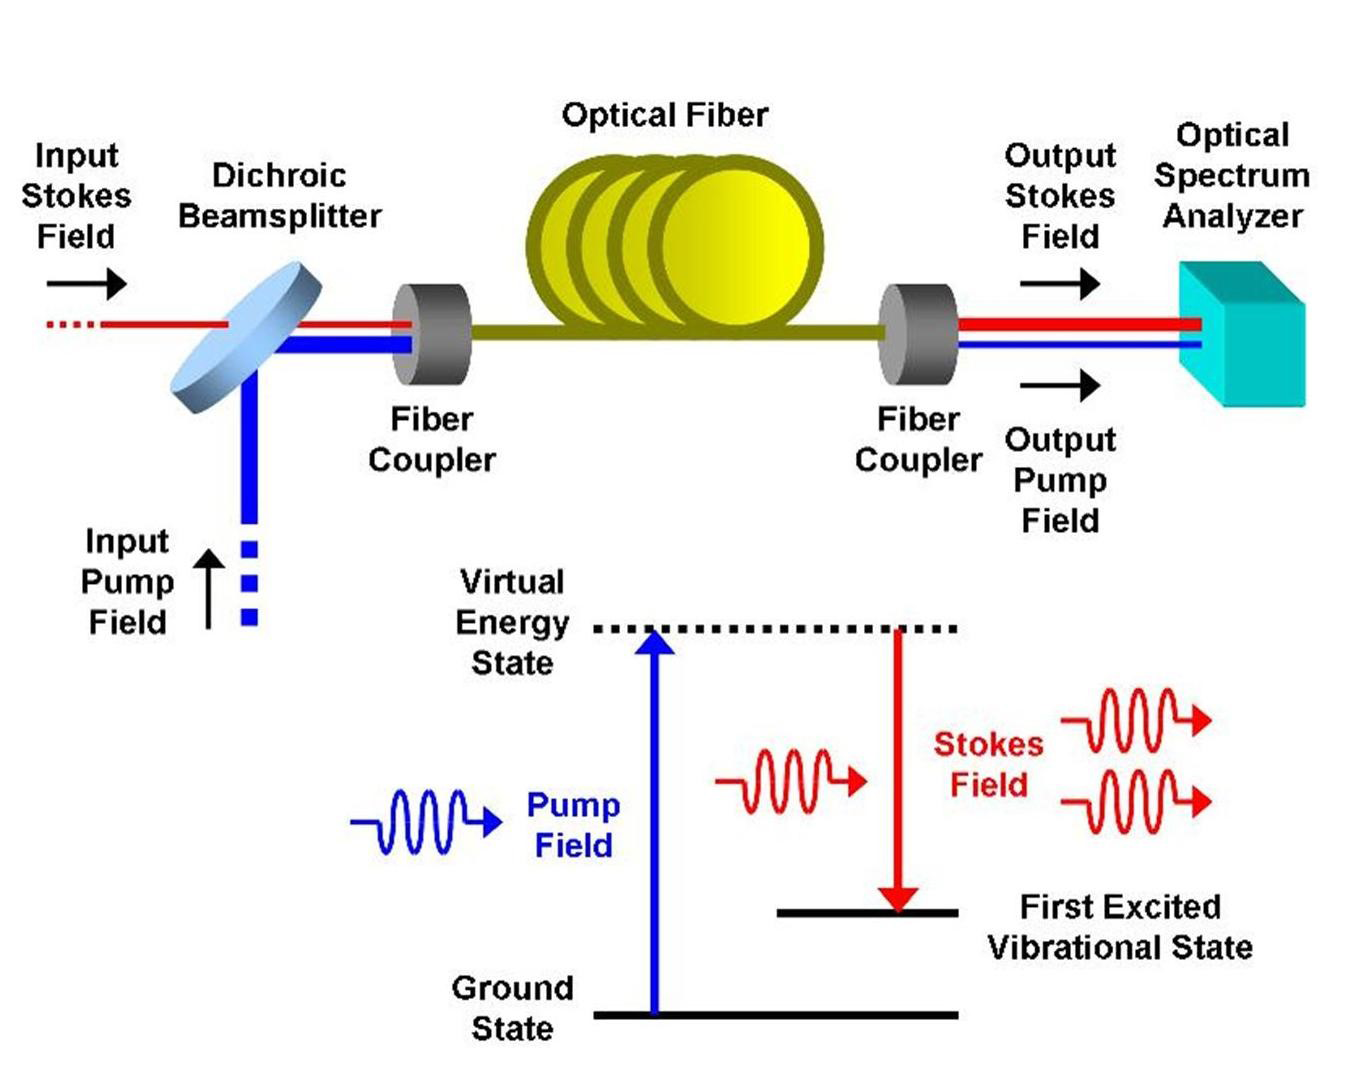
\includegraphics[scale=1]{APL2011/Figure1.png}
\caption{Schematic of the STEAM vibrometer. The principle of the method is three-fold: (1) encoding of the lateral and axial coordinates of the target into the different frequencies and corresponding amplitudes of a spatially dispersed broadband pulse which spectrally interferes with a reference pulse, (2) amplified dispersive Fourier transformation in which the spectrum is mapped into a temporal waveform, time-stretched so that it can be digitized in real time, and simultaneously amplified in the optical domain, and (3) Hilbert transformation on the detected pulse in the digital domain to extract the axial information of the target.}
\label{fig:APL2011_Figure1}
\end{figure}

The interferometrically combined pulses return to the same optics, but are directed via an optical circulator toward the amplified dispersive Fourier transformer (ADFT) \cite{goda2009serial, goda2008amplified, goda2009theory} in which a dispersive fiber with -1200 ps/nm dispersion is optically pumped by four continuous-wave lasers with $\sim$100 mW of optical power at 1470 nm, 1480 nm, 1480 nm, and 1490 nm for distributed Raman amplification. In the dispersive medium, the spectrum of each interfered pulse is stretched and converted into an amplified temporal waveform. This ADFT process is critical for high-speed laser vibrometry because the optical amplification before photon-to-electron conversion overcomes the fundamental trade-off between sensitivity and speed \cite{goda2009serial, goda2009theory}. The pulses are captured by a high-speed photodiode with 15 GHz bandwidth and digitized by a real-time oscilloscope with 16 GHz bandwidth and 50 GS/s sampling rate. Hilbert transformation is applied in the digital domain to each spectrally interfered pulse to obtain the axial information of the target at multiple points along the 1D line. Each pulse acquires one scan and the pulse repetition rate corresponds to the scan rate (frame rate) of the STEAM vibrometer.

The basic capabilities of the STEAM vibrometer (i.e., image pixel number, axial resolution, and dwell time) can be estimated from the parameters of its components. First, the number of image pixels on the target ($ N $) is found from the total dispersion in the dispersive fiber ($ D = \SI{-1200}{ps/nm} $), the optical bandwidth ($ \Delta\lambda = \SI{20}{nm} $), and the sampling rate of the digitizer ($ f_{dig} = \SI{50}{GS/s} $) to be $ N = |D| \cdot \Delta\lambda \cdot f_{dig} = 1200 $ while the number of resolvable points is about 200 from the spectral resolution of the ADFT process [16]. Second, the axial resolution is given by the dynamic range (bit depth) of the digitizer. The axial resolution ($\Delta z$) can be found from the expression, $0.5 \sin(2 \cdot k \cdot \Delta z) = 2^{-n}$, where $k$ is the wavenumber [$k = 2 \pi / (\SI{1590}{nm})$] and $n$ is the bit depth of the digitizer ($n = \SI{8}{bits}$), to be $\Delta z = \SI{0.99}{nm}$. Finally, the dwell time is estimated from the bandwidth of each subpulse ($\SI{20}{nm} /$$\sim$$\num{200}$) and the time-bandwidth product to be $\sim$\SI{30}{ps} (assuming that the subpulses are transform limited).

We evaluated the basic performance of the STEAM vibrometer. In Figure \ref{fig:APL2011_Figure2}a, the temporal waveform of a single interfered pulse captured by the photodiode is compared with the optical spectrum measured by a conventional optical spectrum analyzer. This verifies the equivalence of the two waveforms and hence validates the STEAM vibrometer. As shown in Figure \ref{fig:APL2011_Figure2}b, repetitive pulses (scans) detected by the photodiode indicate that the STEAM vibrometer operates at 36.7 MHz scan rate.

\begin{figure}[htb!]
\centering
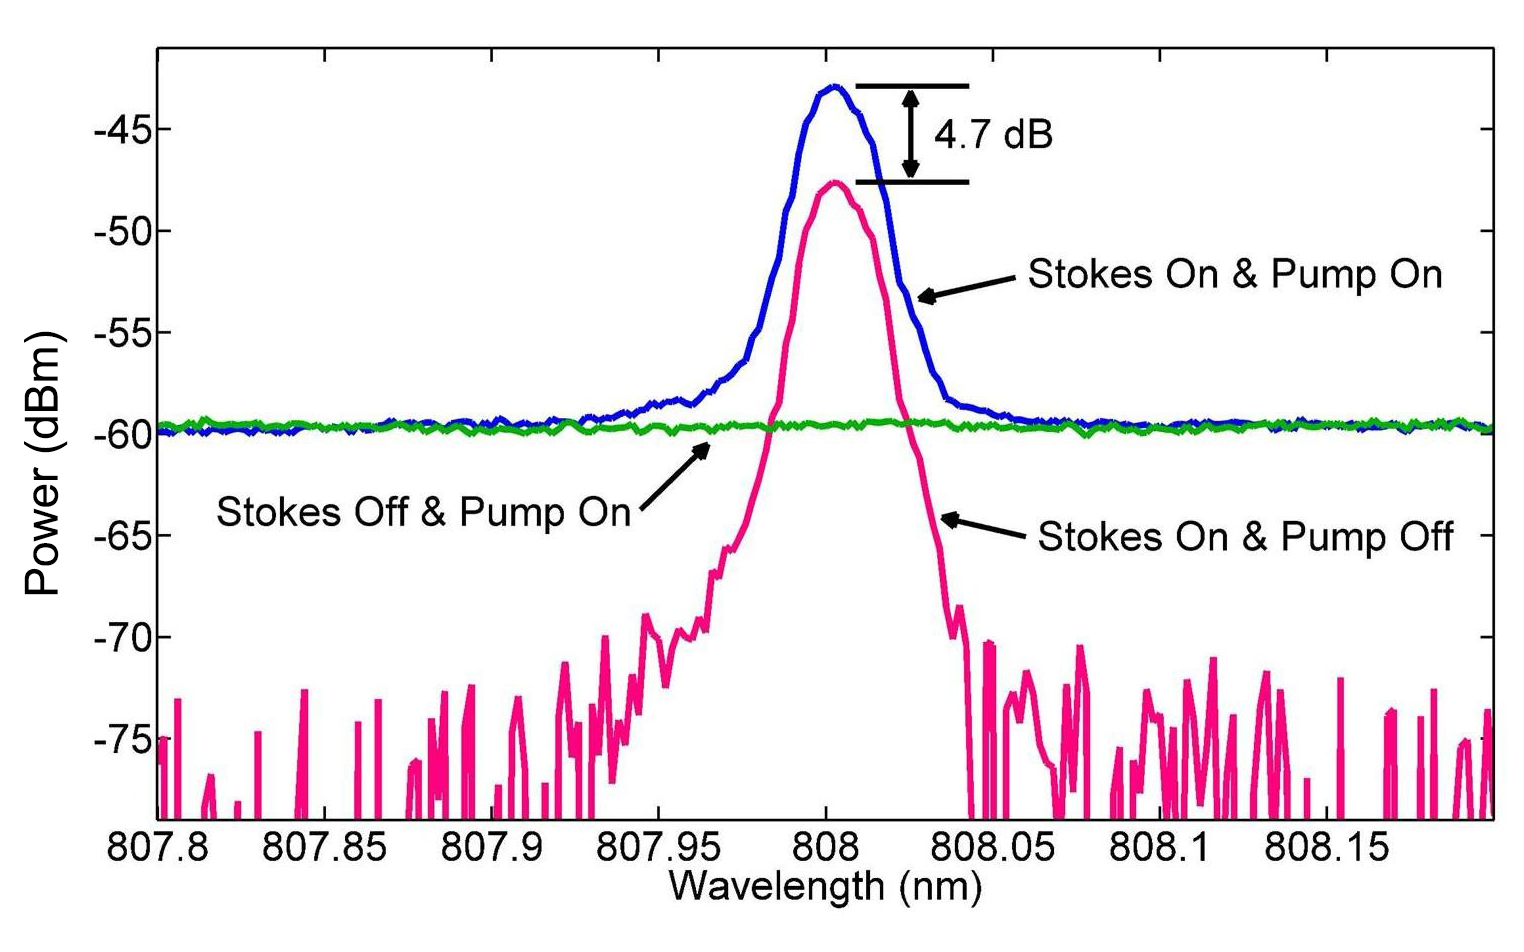
\includegraphics[scale=1]{APL2011/Figure2.png}
\caption{Basic performance of the STEAM vibrometer. (a) Temporal waveform of a single interfered pulse captured by the photodiode in comparison with the optical spectrum measured by a conventional optical spectrum analyzer. (b) Repetitive pulses (scans) with a time interval of 27.2 ns detected by the photodiode indicating that the STEAM vibrometer operates at 36.7 MHz scan rate.}
\label{fig:APL2011_Figure2}
\end{figure}

To show the utility of the STEAM vibrometer, we monitored the performance of an acoustic speaker. For better sensitivity, a thin reflective plate was attached to the diaphragm of the acoustic speaker. The speaker was driven up to 30 kHz (nearly its upper frequency limit). Figure \ref{fig:APL2011_Figure3} shows the 30 kHz surface vibration of the diaphragm captured by the STEAM vibrometer with $\sim$1 nm axial resolution (which agrees with our estimated axial resolution of 0.99 nm).

\begin{figure}[htb!]
\centering
\includegraphics[scale=1]{APL2011/Figure3.png}
\caption{Surface vibration of the acoustic diaphragm captured by the STEAM vibrometer with $\sim$1 nm axial resolution and $\sim$30 ps dwell time. The diaphragm was driven to vibrate at 30 kHz.}
\label{fig:APL2011_Figure3}
\end{figure}

In addition to the amplitude of the surface vibration, we also obtained the velocity of the diaphragm from the axial coordinates of the surface as shown in Figure \ref{fig:APL2011_Figure4}. The Doppler frequency shift in the frequency comb lines caused by the acoustic vibration ($\sim$830 Hz frequency shift) is negligible.

\begin{figure}[htb!]
\centering
\includegraphics[scale=1]{APL2011/Figure4.png}
\caption{Axial velocity of the acoustic diaphragm obtained by the STEAM vibrometer. The diaphragm was driven to vibrate at 30 kHz (the same as in Figure \ref{fig:APL2011_Figure3}).}
\label{fig:APL2011_Figure4}
\end{figure}

In summary, we proposed and demonstrated an optical system that performs high-speed multi-dimensional imaging-based vibrometry and velocimetry with nanometer-scale axial resolution without the need for beam scanning. As a proof-of-concept, we showed real-time 1D imaging of fast acoustic vibrations with 1 nm axial resolution, 1200 image pixels, and 30 ps dwell time at 36.7 MHz scan rate. While we performed 1D cross-sectional imaging in this proof-of-principle demonstration, the technique can naturally be extended to 2D by using a 2D spatial disperser \cite{goda2009serial,tsia2010performance}.

